\documentclass[10pt,a4paper]{article}
\usepackage[margin=1.8cm]{geometry}
\usepackage[T1]{fontenc}
\usepackage{lmodern}
\usepackage{booktabs,tabularx,array}
\usepackage{enumitem}
\usepackage{hyperref}
\usepackage{tikz}
\usetikzlibrary{arrows.meta,positioning}
\usepackage{titlesec}
\usepackage{microtype}

\setlist{nosep,leftmargin=1.2em}
\titlespacing*{\section}{0pt}{6pt}{3pt}
\titlespacing*{\subsection}{0pt}{4pt}{2pt}
\titleformat{\section}{\large\bfseries}{\thesection}{0.6em}{}
\titleformat{\subsection}{\normalsize\bfseries}{\thesubsection}{0.6em}{}
\setlength{\parskip}{2pt}
\setlength{\parindent}{0pt}
\setlength{\emergencystretch}{2em}
\hypersetup{colorlinks=true,urlcolor=blue,linkcolor=black}
\newcommand{\cf}{\textsc{ContractForge}}
\newcommand{\code}[1]{\texttt{\small #1}}

\title{\vspace{-1.2cm}\textbf{\cf: Multi-Agent Generation of Formally Verified\\Lean 4 Code from English Requirements}\\[2pt]
\large Phase 2 -- Mid-Submission Progress Report}
\author{Team AUTOSE-Leaniers\\
\small [Member 1, Bavya Sri Kilari(2025701029), Member 3] \quad [AutoSE]}
\date{\small 6 November 2026\\
\href{https://github.com/Ohshit-ak/AUTOSE-Leaniers}{\nolinkurl{github.com/Ohshit-ak/AUTOSE-Leaniers}}}

\begin{document}
\maketitle
\vspace{-0.8cm}

\section{Project Idea and What Changed Since the Proposal}
\cf{} turns an English software requirements specification (SRS) into Lean~4 code that is machine-checked against the requirements. The pipeline has three layers, and \emph{Lean itself} accepts or rejects the output of each layer before the next one starts:
\begin{itemize}
\item \textbf{L0 (spec agent):} each requirement becomes a Lean specification \code{Spec : Contract Input Output} (a precondition and a postcondition).
\item \textbf{L1 (architect):} the specs are grouped into components, each with a contract, and the proof obligations \textbf{PO1} (consecutive contracts are compatible) and \textbf{PO2} (the composed contract refines the spec) are proved.
\item \textbf{L2 (coding agents):} one agent per component writes an implementation and proves \textbf{PO3}, \code{Contract.Satisfies c f}.
\end{itemize}
A soundness theorem in the framework (\code{Contract.system\_sound}) combines PO1--PO3 into end-to-end correctness. The framework library is Lean core only (no Mathlib), so builds stay fast.

\begin{figure}[h]
\centering
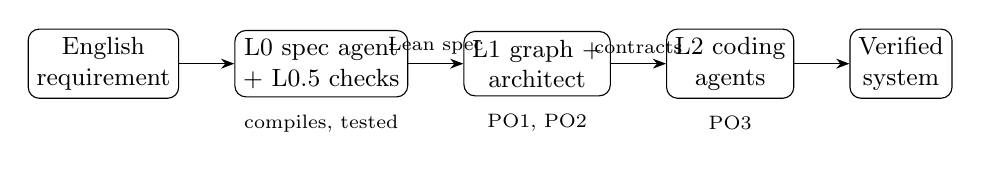
\begin{tikzpicture}[node distance=7mm,
  box/.style={draw,rounded corners,align=center,minimum height=8mm,inner sep=3pt,font=\small},
  lab/.style={font=\scriptsize,align=center},
  >=Stealth]
\node[box] (req) {English\\requirement};
\node[box,right=of req] (l0) {L0 spec agent\\+ L0.5 checks};
\node[box,right=of l0] (l1) {L1 graph +\\architect};
\node[box,right=of l1] (l2) {L2 coding\\agents};
\node[box,right=of l2] (sys) {Verified\\system};
\draw[->] (req)--(l0); \draw[->] (l0)--node[lab,above]{Lean spec} (l1);
\draw[->] (l1)--node[lab,above]{contracts}(l2); \draw[->] (l2)--(sys);
\node[lab,below=1mm of l0] {compiles, tested};
\node[lab,below=1mm of l1] {PO1, PO2};
\node[lab,below=1mm of l2] {PO3};
\end{tikzpicture}
\caption{The \cf{} pipeline. Each arrow is gated by the Lean type checker.}
\end{figure}

\textbf{Changes to the original proposal.}
(1) A large part of the time went into making L0 reliable, because every later layer depends on it; L0 is now frozen (v10.1).
(2) In L1, contracts are written over a \emph{harness-generated message type} instead of a shared \code{World} record: one \code{World $\to$ World} step cannot satisfy conflicting operations such as login and logout.
(3) \code{SystemSpec} is generated by the harness as the conjunction of the L0 specs, and every theorem statement (trace, PO1, PO2) is written by the harness. The model only writes the contract bodies, so it cannot weaken what has to be proved.
(4) Cyclic component groups are merged rather than rejected, because stopping left the main benchmark with nothing to run.
(5) To get a first L2 number before this deadline we added a second, simpler L1/L2 path next to the graph one: each L0 spec on its own is split into exactly two chained contracts (\code{Input $\to$ Mid $\to$ Output}), and then one coder per contract proves PO3. The graph path is still the main design; the per-spec path is what L2 has been run on so far.

\section{Architecture and Implementation Plan}
The system is a Python harness around a small Lean 4 library.

\textbf{Lean framework} (\code{framework/}): \code{Contract.lean} (the \code{Contract} type, PO1--PO3, sequential composition), \code{Soundness.lean} (\code{seq\_sound}, \code{refines\_sound}, \code{system\_sound}), \code{Chain.lean} (chains of $n$ components), \code{Strings.lean} (decidable string-format helpers), and a \code{discharge\_po} tactic that tries \code{simp\_all}, \code{omega}, \code{grind} and \code{decide}. \code{discharge\_po [A, B]} also unfolds the named contracts (the plain version left user contracts opaque and could never close PO1/PO2).

\textbf{Harness} (\code{harness/}): a single entry point \code{main.py} with stages \code{parse $\to$ spec $\to$ check $\to$ graph $\to$ arch $\to$ code}. Its main parts:
\begin{itemize}
\item \code{req\_parser.py}: a rule-based, LLM-free SRS parser. The same XML always gives the same JSON, and every dropped sentence is kept with the rule that dropped it.
\item \code{agents/base.py}: a shared generate $\to$ check $\to$ repair loop used by every agent. Repairs show only the earliest error layer (syntax, names, types, proofs), mechanical fixups run first, and attempts that weaken the spec are rejected. For L1/L2, re-declared locked names are stripped, and \code{agents/autoprove.py} tries generic proof scripts on each PO before asking the model again.
\item \code{validate.py} (L0.5): checks beyond compilation: vacuity (\code{post} must reject a changed output), parser facts such as runtime bounds, data-field tests built from the SRS rules, and a negative check in which the model names one forbidden behaviour that Lean must show the spec rejects.
\item \code{req\_graph.py}, \code{arch\_lean.py}, \code{agents/architect\_agent.py}: the L1 requirements graph and architect (Section~3).
\item \code{agents/coding\_agent.py}, \code{code\_lean.py}: the L2 coder for graph architectures (Section~3).
\item \code{e2e\_l1l2.py}, \code{agents/chain\_architect.py}, \code{agents/chain\_coder.py}: the per-spec L1/L2 path, run on a finished L0 run; it can be split into shards that run as parallel GPU jobs.
\end{itemize}
Models: a local Qwen~2.5~7B (Q4\_K\_M, llama.cpp) on a university GPU cluster is the main model; DeepSeek, Groq and Gemma are supported through the same \code{call\_llm} interface. Runs are seeded and repeatable (\code{--repeat N}), and \code{evaluation/compare\_runs.py} reports mean (min--max) over repetitions, declaring a change ``better'' or ``worse'' only when it exceeds the run-to-run spread. \code{evaluation/summarize\_e2e.py} gives the L1, L2 and end-to-end counts of a per-spec run.

\section{Progress Completed}
\subsection{L0: requirements $\to$ Lean specifications (done, frozen at v10.1)}
The parser extracts 75 entries from the gamma~j SRS (35 requirements, 20 data constraints, 20 use cases; 219 statements dropped with reasons). A second SRS (video search, 21 entries) is used as a sanity check. Table~\ref{tab:l0} shows how the compile rate moved with each version of the prompt and repair loop.

\begin{table}[h]
\centering\small
\begin{tabularx}{\linewidth}{@{}lXr@{}}
\toprule
Version & Change & Entries compiling (of 75)\\
\midrule
No Lean check & first prompt, no repair loop & 0 (by hand)\\
v1 & hardened prompt (templates, Lean 3 syntax banned) & 30\\
v2 & prompt v2 + conversational repair loop & 55\\
v4 & staged repair, witness search, 16k context & 65\\
v8 & vacuity fix, fixups, hints, negative-check parsing & 68\\
v10.1 (\(\times\)3 seeds) & string library, name suggestions, truncation guard & 67.0 (66--68)\\
\bottomrule
\end{tabularx}
\caption{L0 on gamma~j with Qwen~2.5~7B. Compiling is necessary but not sufficient, which is why L0.5 exists.}
\label{tab:l0}
\end{table}

Over three seeds, v10.1 gives 61 L0.5 passes (57--63) against 53.3 (51--56) for v8, with 2.16 attempts per entry (v8: 2.58). Most of that gain is a scoring change (no ``\code{pre = True}'' flag when the requirement states no precondition), so on equal scoring the pass rates are about equal (about 64 vs.\ 61). We report this rather than the larger number. A single run moves by about $\pm5$ passes on its own, which is why we moved to three-seed comparisons.

\subsection{L1: requirements graph and architecture (done, evaluated on gamma~j)}
\textbf{Graph (no LLM).} \code{req\_graph.py} builds a deterministic graph in which operations are L0 specs and entities come from \code{Domain.lean}, the data dictionary, a glossary and a synonym file. Edges are write$\to$read dataflow and use-case links. Connected groups become systems, large groups are split with Louvain clustering, cycles are listed and then merged, and the topological order gives the chain of components. On gamma~j this gives 8 groups, 9 components, 6 cycles (1 merged set) and 184 edges; 47.2\% of fields map to a domain entity (116/246).
\textbf{Architect.} For each operation the model writes only \code{<C>\_pre\_<op>} and \code{<C>\_post\_<op>}. The harness checks that the contract compiles, is satisfiable on the L0 example, is not vacuous, and satisfies the trace obligation (\code{pre} assumes no more than the L0 \code{pre}; under it \code{post} implies the L0 \code{post}). PO1 and PO2 proofs are generated mechanically from the ownership map, so they scale: all 67 compiling specs as one system check in about 12\,s. Three modes exist: pipeline (default), agent (model calls the tools) and no-graph (baseline, the model decomposes the system itself).

\begin{table}[h]
\centering\small
\begin{tabular}{@{}lcc@{}}
\toprule
Qwen~2.5~7B, group \code{AccountSys} (48 ops), 3 seeds & graph & no graph\\
\midrule
\code{Arch.lean} compiles & 3/3 & 1/3\\
Contracts satisfiable and non-vacuous & 100\% & 33\%\\
Trace obligations proved & 99\% & 33\% (0--99)\\
PO1 proved & 100\% & 33\%\\
PO2 proved & 0/3 & 0/3\\
Minutes per run & 12.2 & 4.6\\
\bottomrule
\end{tabular}
\caption{L1 (graph path) results. The graph variant produced a valid decomposition in every run; without the graph, 2 of 3 runs returned a decomposition the harness rejected.}
\label{tab:l1}
\end{table}

In graph mode, 96 of 98 obligations are proved in every run. Exactly one \code{trace\_post} fails per run (\code{3.5.3/S2} in two runs, \code{3.1.3/S1} in one), and PO2 fails with it, since it needs every trace first. With only three repetitions and a bimodal baseline, the comparison tool calls the difference ``within noise'', so the advantage of the graph is indicative, not established.

\subsection{L2: implementation and PO3 (first end-to-end runs, per-spec path)}
The L2 coding agent takes a locked contract and generates an implementation plus a proof of \code{Contract.Satisfies c f} (PO3), using the same generate--check--repair loop. For the graph path, the coder (\code{coding\_agent.py}, \code{code\_lean.py}, the \code{code} stage in \code{main.py}, about 700 lines of tests) is merged into \code{main} but has not been run on the gamma~j architecture yet, since no graph architecture is accepted (PO2 above).

On the per-spec path we ran L1 and L2 end to end on every L0 spec that compiled and was accepted by L0.5 (single run, seed 42, Qwen~2.5~7B). The first attempt (v1) proved nothing in L1 (0/61 on gamma~j, 0/14 on video search): every reply re-declared the locked \code{Input}/\code{Output}/\code{Spec}, many component types did not chain, and \code{discharge\_po} could not unfold the user's contracts. After fixing these (v2), we get Table~\ref{tab:e2e}. ``End to end'' means L1 proved, every L2 component proved, and the combined file checked by Lean once more.

\begin{table}[h]
\centering\small
\begin{tabular}{@{}lcccc@{}}
\toprule
Per-spec path, v2 & specs in & L1 (PO1+PO2) & L2 components (PO3) & end to end\\
\midrule
gamma~j & 61 & 29/61 & 48/58 & 19/61\\
video search & 14 & 9/14 & 16/18 & 7/14\\
\bottomrule
\end{tabular}
\caption{First L1+L2 results (one run each; gamma~j took 65 min of model time, run as parallel shards). On gamma~j: requirements 12/27, use cases 7/17, data constraints 0/17 end to end.}
\label{tab:e2e}
\end{table}

These numbers look better than they are. 12 of the 19 gamma~j passes (and 3 of 7 on video search) have a \emph{pass-through} first component that only copies its input (\code{m.x = i.x}), so they verify but do not really decompose anything; about 7 are real two-step designs. L2 itself is the easier step: once L1 holds, most components get a proved implementation.

\subsection{Evaluation assets and tests}
\code{benchmark/gammaj/} holds a hand-written gold L0 file (25 specs, all with satisfiability witnesses, ambiguities marked) and a reviewed \code{Domain.lean}. The unit tests cover the parser, the negative check, harness regressions, L0 versions v9 and v10, the requirements graph, every L1 tool and the L2 coder (128 tests passing on \code{main}). The repository has 76 commits between 19 October and 6 November; the work was done on branches (\code{l0-v10}, \code{l1-graph-contracts}, \code{l1\_runs}, \code{feat/l2-coding-agent}, \code{fix/l0-spec-quality}), and all of them are now merged into \code{main} (PRs \#1 and \#2).

\section{Preliminary Demonstration}
Run on the gamma~j SRS (an online shop with accounts, a cart, products and orders). Example flow for the requirement ``log in'':
\begin{enumerate}
\item L0 produces \code{Spec} with \code{Input} (credentials, a list of accounts) and \code{Output} (\code{signedIn}), where \code{post} says \code{signedIn = true $\leftrightarrow$ $\exists$ a $\in$ accounts, \ldots}, and Lean proves a satisfiability \code{example}.
\item L0.5 checks that \code{post} rejects a changed output, and the model's forbidden example (wrong password $\to$ signed in) is shown to be rejected by \code{decide}. This catches the first-generation login spec, which accepted every login.
\item L1 assigns the spec to a component, the model writes \code{Account\_pre\_login} and \code{Account\_post\_login}, and the harness proves the trace obligation and PO1 for consecutive components; PO2 for the chain is attempted but has failed in every run so far (Section~5).
\item On the per-spec path, a spec such as ``sales person removes a product'' (\code{UC-sales-person-remove-product}) goes through L1 and L2 and comes out as one Lean file with the spec, two contracts, two implementations and all three POs proved. Even here the split is shallow: the first component does the filtering and the second only copies it on.
\end{enumerate}
Every run writes self-contained, checkable output: each Lean file starts with \code{import ContractForge} and compiles with \code{lake env lean <file>} from the repository root; \code{arch.json} and \code{l1l2.json} record every obligation, attempts and errors; \code{Arch.lean} marks unproved obligations as \code{-- NOT PROVED:} comments.

\section{Known Failures and Limitations}
\begin{itemize}
\item \textbf{Compiling is not correctness.} An L0 spec that compiles and passes L0.5 can still say too little (``confirm orders'' gives a weak \code{post}). One negative example is weak evidence, and it catches a \code{post} that accepts too much, not one that rejects valid outputs. We therefore review specs by hand, but only some of them so far.
\item \textbf{L0 failures that persist:} \code{5.5/R1} and \code{DD-shipping-date} fail in every version; \code{DD-credit-card-expiry-date}, \code{DD-location} and the checkout use case fail in about two of three runs. Seven L0 specs do not compile and are therefore excluded from L1. Typical causes are invented library functions (\code{List.nth}, \code{String.substring}), type errors on tuples, and date formats.
\item \textbf{L1 graph path: PO2 is proved in no run.} One \code{trace\_post} obligation fails per run, with the error ``Expected type must not contain free variables''. We have not yet investigated the cause, and fixing it would likely let the system be accepted.
\item \textbf{L1 contracts can be trivial.} A contract equal to the L0 conditions makes every obligation easy, and nothing yet rewards a contract that says more than the requirement. On the per-spec path the same problem shows up as pass-through components (15 of the 26 end-to-end passes); there is no semantic check that rejects them yet.
\item \textbf{Data constraints cannot be split.} All 17 gamma~j data constraints fail per-spec L1: a data constraint is one validity check, and the model moves the check into the second component's \code{pre}, which makes PO2 false. These specs should skip L1 or be allowed one component. Also, \code{Mid} must carry every field the second component needs (video search \code{REQ-1} fails because of this).
\item \textbf{Graph quality depends on inputs.} Only 47.2\% of fields map to a domain entity; session state (\code{signedIn}, \code{cookie}) has no entity. Seven of the eight groups are single data-dictionary fields and are skipped by L1 (fewer than two compiling specs), so the graph path has so far been evaluated on one system.
\item \textbf{Limited evidence.} Three seeds per condition for L0 and graph L1, a single run for the per-spec L1/L2 results, one model size (7B), one main SRS. The video-search SRS was looked at while writing v9, so it is not a held-out test. L2 failures (often one of the two components fails) are not analysed yet.
\item \textbf{Model dependence.} Qwen~2.5~7B is small. A larger model (Gemma through the API) is planned for a single comparison run but has not been run.
\end{itemize}

\section{Remaining Work}
\begin{enumerate}
\item \textbf{Run L2 on the graph path} (the \code{code} stage in \code{main.py}) once a gamma~j architecture is accepted, and report PO3 pass rate, attempts and time per component with three seeds. [Add date/owner.]
\item \textbf{Fix the failing L1 trace} (\code{3.5.3/S2}, \code{3.1.3/S1}) so that PO2 and \code{system\_sound} can be proved for the full system, then rerun the graph vs.\ no-graph comparison.
\item \textbf{Per-spec path:} a semantic L1 check that rejects pass-through and copy-of-\code{Spec} components, one-component handling for data constraints, the \code{Mid}-fields rule in the prompt, a look at the L2 failures, and three seeds instead of one.
\item \textbf{Second benchmark system} (\code{benchmark/bank\_ledger/}) and a held-out SRS, so results do not rest on one document.
\item \textbf{Stronger contracts in L1:} reward contracts that add constraints beyond the L0 text, and relate operations to one another.
\item \textbf{Model comparison:} one Gemma run (and DeepSeek if a key is available) to check how much of the failure rate is due to the 7B model.
\item \textbf{Re-verification and reporting:} \code{harness/reverify.py} (recheck a finished run from its JSON), a \code{requirements.txt}, and \code{evaluation/metrics.py} with one result record per run.
\item \textbf{Housekeeping:} wire the per-spec path into \code{main.py} (or drop it once the graph path works), review more generated specs by hand, and revoke an API key that was committed to the history early on.
\end{enumerate}

\section{Summary}
Beyond a proposal, the project has a working Lean framework with a soundness theorem, a deterministic parser, an L0 agent that compiles about 89\% of gamma~j entries with a 7B local model (up from 0 without a repair loop), an L1 graph and architect that prove 96 of 98 obligations per run and are more reliable with the graph than without it, and a first end-to-end L1+L2 result: 19 of 61 gamma~j specs and 7 of 14 video-search specs are fully verified from spec to implementation, though many of these use a trivial first component. The main open risks are the single failing L1 obligation that blocks PO2 on the graph path, and the weak decompositions on the per-spec path.

\end{document}
